\documentclass{standalone}
\usepackage{tikz}
\usepackage{ctex,siunitx}
\setCJKmainfont{Noto Serif CJK SC}
\usepackage{tkz-euclide}
\usepackage{amsmath}
\usetikzlibrary{patterns, calc}
\usetikzlibrary {decorations.pathmorphing, decorations.pathreplacing, decorations.shapes,}
\begin{document}
\small
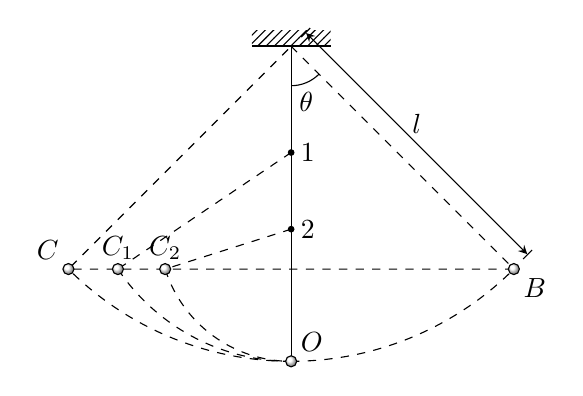
\begin{tikzpicture}[>=stealth,scale=1.0]
  \fill [pattern = north east lines] (-.5,0) rectangle (.5,0.2);
  \draw[thick] (-.5,0)--(.5,0);
  \draw (0,0)--(0,-4);
  \draw (0,-.5) arc (-90:-45:.5)node[midway,below]{$\theta$};
  \draw [dashed] (0,0)--(-45:4)--(-135:4)--(0,0);
  \draw[dashed] (0,-4) arc (-90:-45:4);
  \draw[dashed] (0,-4) arc (-90:-135:4);
  \draw[dashed] (0,-1.3486) --(-2.2,-4/1.414);
  \draw[dashed] (0,-2.3217) --(-1.6,-4/1.414);
  \draw[dashed] (-2.2,-4/1.414) arc(-146.074:-90:2.6514);
  \draw[dashed] (-1.6,-4/1.414) arc(-162.426:-90:1.6783);
  \draw[fill=black] (0,-1.3486) circle (1pt)node[right]{1};
  \draw[fill=black] (0,-2.3217) circle (1pt)node[right]{2};
  \draw [ball color=white] (-45:4) circle (2pt)node[below right]{$B$};
  \draw [ball color=white] (-135:4) circle (2pt)node[above left ]{$C$};
  \draw [ball color=white] (0,-4) circle (2pt)node[above right]{$O$};
  \draw [ball color=white] (-2.2,-4/1.414) circle (2pt)node[above]{$C_1$};
  \draw [ball color=white] (-1.6,-4/1.414) circle (2pt)node[above]{$C_2$};
  \draw [|<->|](.18,.18) -- (2*1.414+.18, -2*1.414+.18) node [midway,above]{$l$};
\end{tikzpicture}
\end{document}